\chapter{Inferential Statistics}

\section{Two-way ANOVA}
\subsection{Problem Statement}

Many customers believe that the product lines in each applied segment will have different numbers of cores, so perform ANOVA testing to check if there is a relationship between \texttt{Product\_Collection} and \texttt{Vertical\_Segment} to \texttt{nb\_of\_Cores}.

\begin{lstlisting}[language = R]
  CPUs_ANOVA_input <-
  get_valid(
    CPUs_selected %>%
      filter(Product_Collection %in% c("Core", "Legacy") &
            Vertical_Segment %in% c("Desktop", "Embedded", "Mobile")) %>%
      select(Product_Collection, Vertical_Segment, nb_of_Cores)
  ) 
\end{lstlisting}

\begin{figure}[ht]
  \centering
  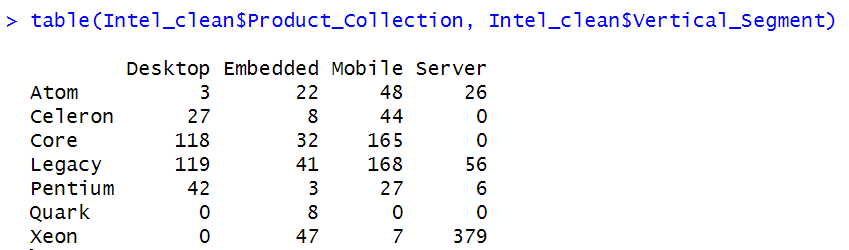
\includegraphics[width=14cm]{img/1.png}
  \vspace{0.5cm}
  \caption{Data Partition based on \texttt{Product\_Collection} and \texttt{Vertical\_Segment}}
\end{figure}

\subsection{Tests of Conditional Hypotheses}
Before ANOVA test, let us test whether initial conditions are satisfied.
\begin{enumerate}
  \item Testing whether \texttt{nb\_of\_Cores} is normal-distributed ($H_0$) or not ($H_1$). Since $p_{\mathrm{value}}< 0.05$, we reject $H_0$ i.e. \texttt{nb\_of\_Cores} is not normal-distributed.
        \begin{lstlisting}[language=R]
    library(nortest)
    shapiro.test(CPUs_ANOVA_input$nb_of_Cores)

    # Output: 	Shapiro-Wilk normality test

    # data:  CPUs_ANOVA_input$nb_of_Cores
    # W = 0.62213, p-value < 2.2e-16
  \end{lstlisting}

        \begin{figure}[ht]
          \centering
          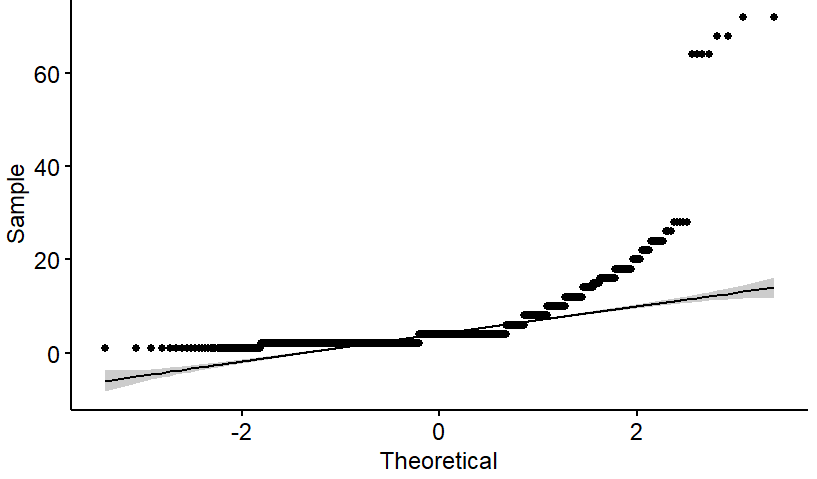
\includegraphics[width=0.6\textwidth]{img/5.png}
          \vspace{0.5cm}
          \caption{Q-Q plot returned by \texttt{ggqqplot(nb\_of\_Cores)}. Observed values are far away from normal expectation.}
        \end{figure}

  \item Testing whether the variances are equal $(H_0)$ or there exist two groups of different variances $(H_1)$. Since $p_{\mathrm{value}} = 1.339e-07 < 0.05$, we reject $H_0$.
        \begin{lstlisting}[language=R]
    library(car)
    leveneTest(CPUs_ANOVA_input$nb_of_Cores ~ 
                CPUs_ANOVA_input$Product_Collection * 
                CPUs_ANOVA_input$Vertical_Segment)

    # Output
    # Levene's Test for Homogeneity of Variance (center = median)
    # Df F value    Pr(>F)    
    # group   5  8.2835 1.339e-07 ***
    #    645    
  \end{lstlisting}
\end{enumerate}

Thus, \texttt{nb\_of\_Cores} is not normally distributed, and the variances of the groups are not equal. However, the sample size is large (more than $30$). Therefore, we can disregard these violations.

\subsection{ANOVA Test}

Our objective is to examine the impact of the two factors \texttt{Product\_Collection} and \texttt{Vertical\_Segment} on \texttt{nb\_of\_Cores}. Since this is a large sample, even though the sample violates the assumptions of normal distribution and homogeneity of variances, the two-factor ANOVA method can still be applied. However, the results are only for reference. For more accurate results, other methods can be used.

\begin{lstlisting}[language=R]
  av <- aov(nb_of_Cores ~ 
              Product_Collection * 
              Vertical_Segment,
            data = CPUs_ANOVA_input)
  summary(av)
  # Output
  #                                      Df Sum Sq Mean Sq F value   Pr(>F)    
  #Product_Collection                    1   94.6   94.64  46.895 1.75e-11 ***
  #Vertical_Segment                      2  198.2   99.08  49.093  < 2e-16 ***
  #Product_Collection:Vertical_Segment   2   27.4   13.71   6.795   0.0012 ** 
  #Residuals                           645 1301.7    2.02    
\end{lstlisting}

From the mean squares, we see that the effects of \texttt{Product\_Collection} and \texttt{Vertical\_Segment} appear to be similar, and both effects are statistically significant, as the $p$-values for both factors are very low. Specifically, for \texttt{Product\_Collection}, the hypotheses are the average number of CPU cores in the two product types, Core and Legacy, are the same ($H_0$) or different ($H_1$). For \texttt{Vertical\_Segment}, they are the average number of CPU cores in the application segments Desktop, Embedded, and Mobile are the same ($H_0$) or at least two segments have different average numbers of CPU cores ($H_1$). Both $H_0$ hypotheses are rejected. We conclude that the average number of CPU cores is different for different product lines (\texttt{Product\_Collection}) and application segments (\texttt{Vertical\_Segment}), so the average number of CPU cores depends on the product line and application segment.